\documentclass{article}
\usepackage{graphicx}

\begin{document}

\title{Art \& History Museum HTML}
\author{
  Ahmed Raof Abdel Halim\\
  \texttt{github.com/AhmedRaof}
  \and
  Saif Al Eslam Hossam Mahmoud Shalaby\\
  \texttt{github.com/0xSh3rl0ck}
  \and
  Mohamed Raafat Ebrahim Ramadan\\
  \texttt{https://github.com/A4Te}
  \and
  Abdel Rahman Ashraf \\
  \texttt{github.com/abdelrahmanashraf31}
  \and
  Omar Ayman Mohamed \\
  \texttt{github.com/Maro-o}
  \and
  Eslam Saeed Goda \\
  \texttt{github.com/Eslamsaed115}
}
\date{}
\maketitle
%%%%%%%%%%%%%%%%%%%%%%%%%%%%%%%%%%%%%%%%%%%%%%%%%%%%%%%%%%%%%%%%%%%%%%%
\begin{abstract}
'We created an art and exhibition-based beautiful museum website with awesome unique elements. It shows the artistic statues that exist around the world. Through our website, you can have a glance at past exhibitions and enjoy arts from all over the world. Videos and photo galleries are still available to view online.
\end{abstract}
%%%%%%%%%%%%%%%%%%%%%%%%%%%%%%%%%%%%%%%%%%%%%%%%%%%%%%%%%%%%%%%%%%%%%%%
\section{Website Header}
In our website header we have nav-bar which contains many tabs such as:
\begin{itemize}
\item Translation Option from arabic to english and vice versa
\item Visit
\item Exhibitions
\item Collections
\item About
\item Contact
\item Search Button
\item Get a Ticket (Button)
\end{itemize}
\subsection{Search Button}
We added a feature to the search button that shows recent events when clicked on and allows the user to search for old ones. You can check all of these in Fig \ref{fig:header}. 
\begin{figure}
	\centering
	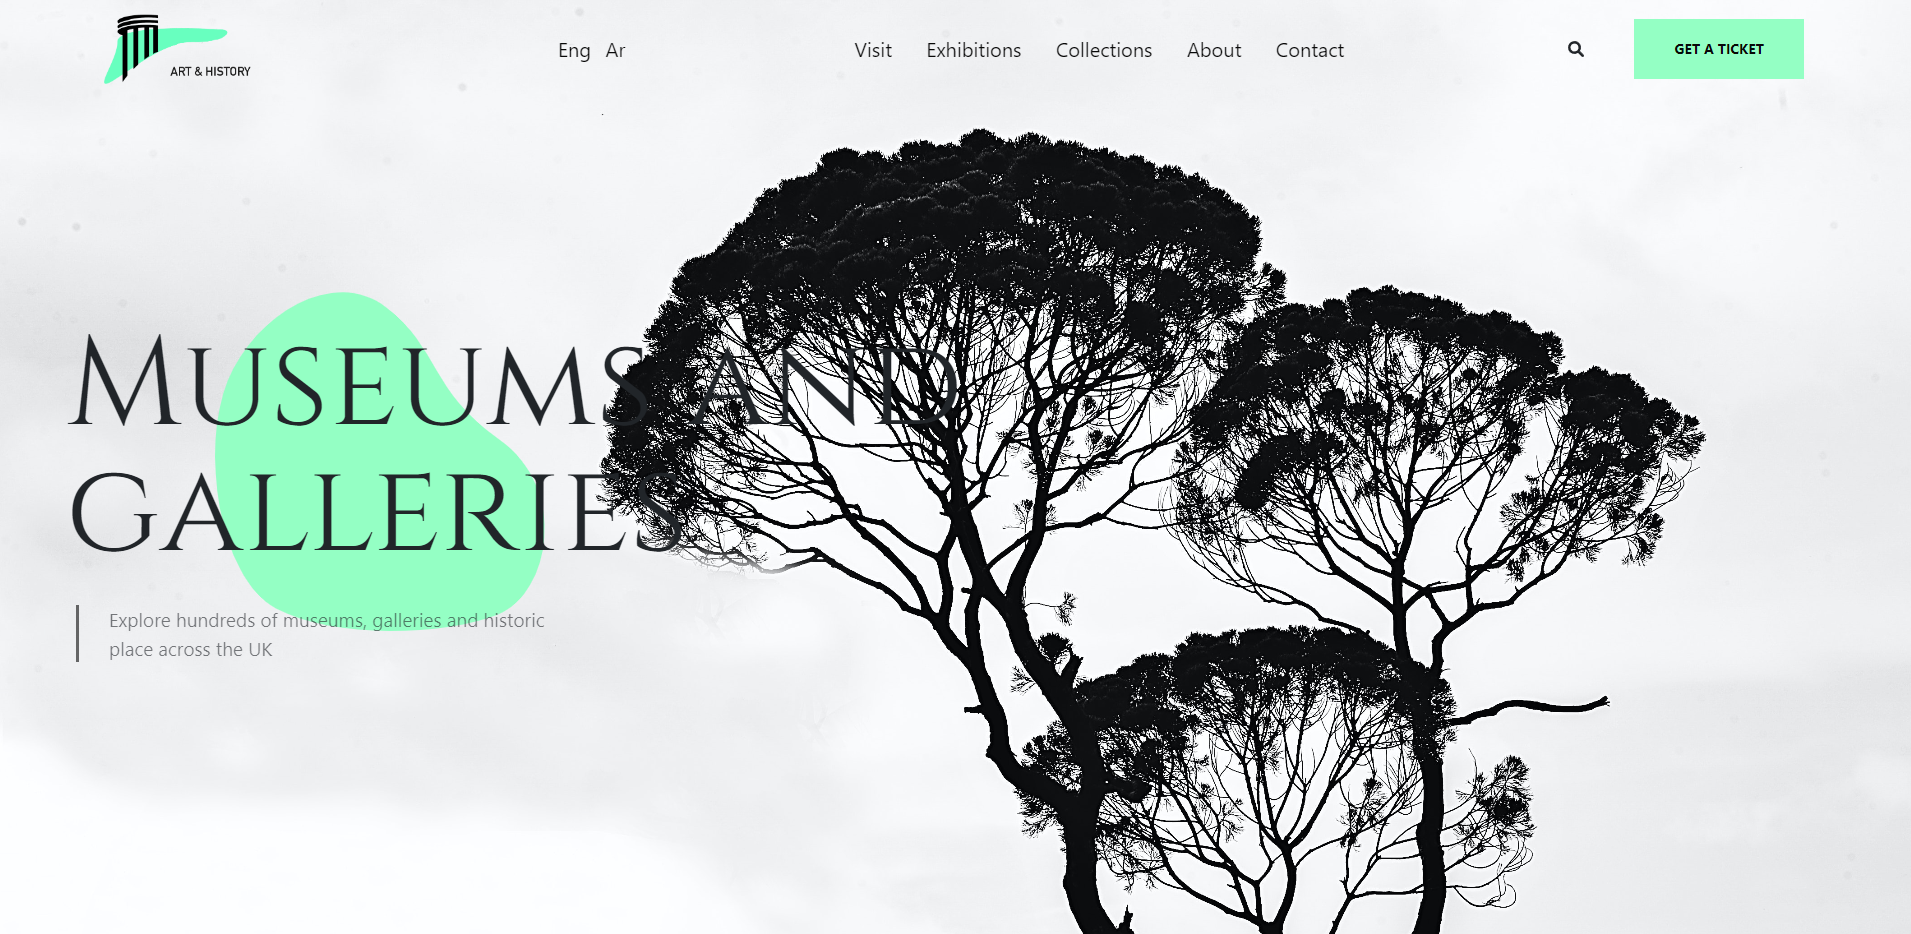
\includegraphics[width=\linewidth]{img/header.PNG}
	\caption{Header}
	\label{fig:header}
\end{figure} 
%%%%%%%%%%%%%%%%%%%%%%%%%%%%%%%%%%%%%%%%%%%%%%%%%%%%%%%%%%%%%%%%%%%%%%%
\section{Museum of Art}
In this section, we are illustrating some information about the world's leading museum of art. We announce the opening times, online booking methods, and provide location services.  You can check this on Fig \ref{fig:leading}. 
\begin{figure}
	\centering
	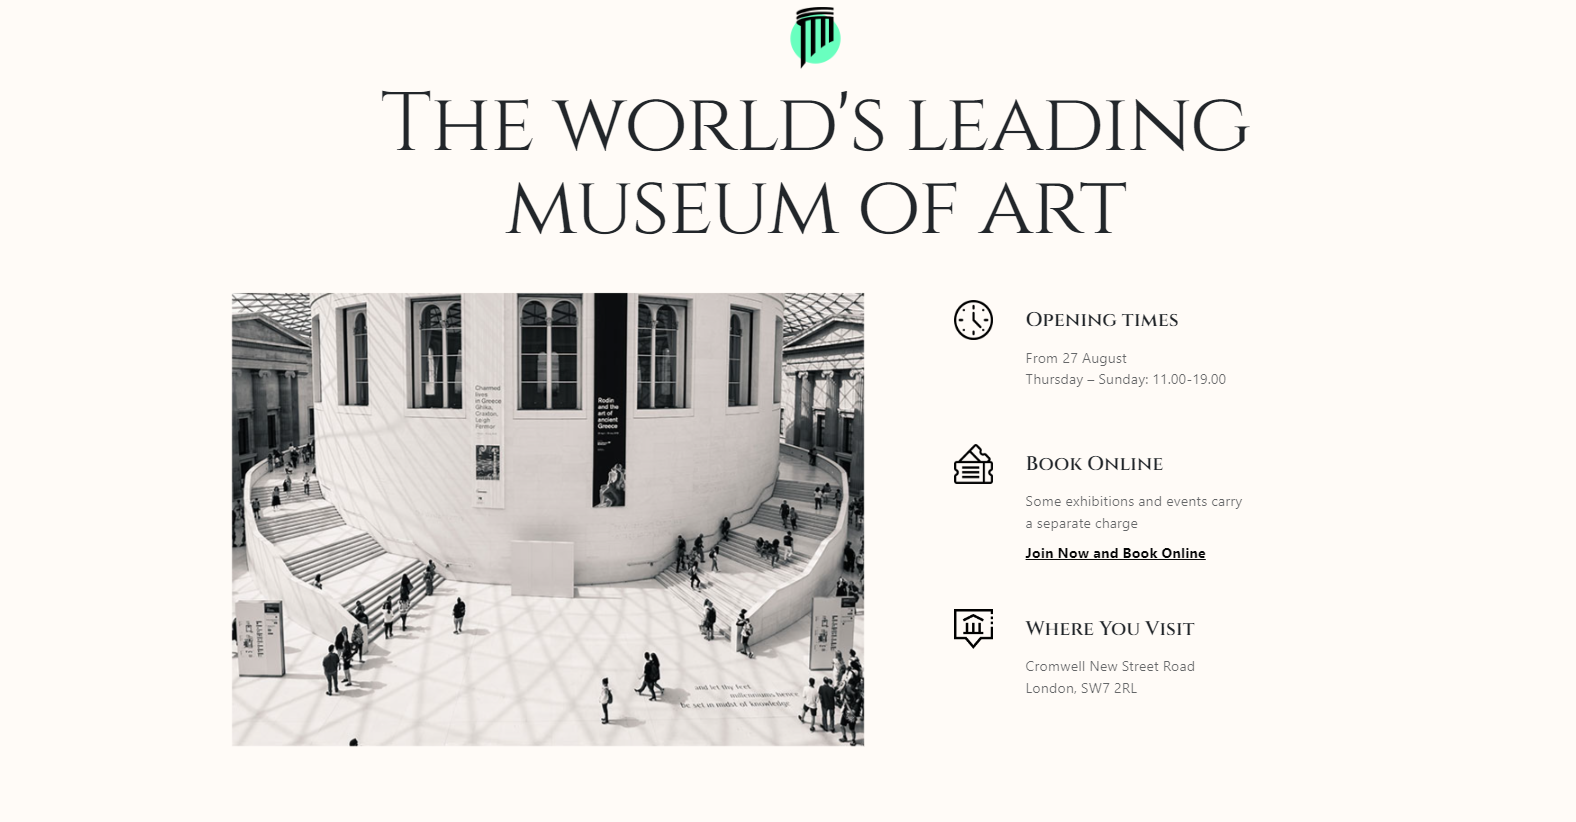
\includegraphics[width=\linewidth]{img/leading.PNG}
	\caption{Header}
	\label{fig:leading}
\end{figure} 
%%%%%%%%%%%%%%%%%%%%%%%%%%%%%%%%%%%%%%%%%%%%%%%%%%%%%%%%%%%%%%%%%%%%%%%
\section{Upcoming Events}
We will inform the visitors with the necessary information about the upcoming events, such as the date, location, and event speakers. Fig \ref{fig:upcoming}.
\begin{figure}
	\centering
	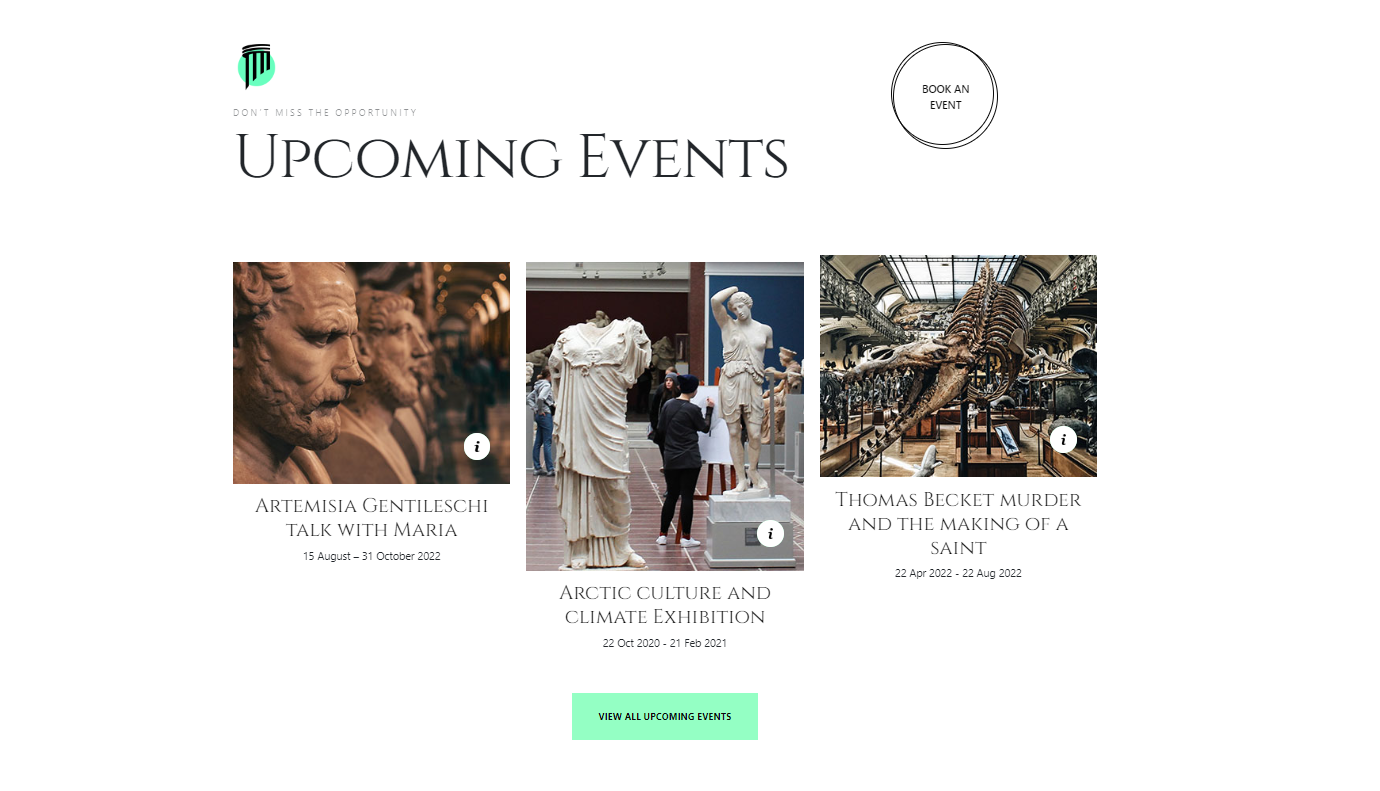
\includegraphics[width=\linewidth]{img/upcoming.PNG}
	\caption{Header}
	\label{fig:upcoming}
\end{figure} 
%%%%%%%%%%%%%%%%%%%%%%%%%%%%%%%%%%%%%%%%%%%%%%%%%%%%%%%%%%%%%%%%%%%%%%%
\section{Safety Measures}
Safety of our visitors is a priority so, we provide a 3 steps to ensure their safety:
\begin{itemize}
\item ensure social distancing.
\item we provide an online method for booking tickets
\item We created a virtualized version of the museum on the website.
\end{itemize}
see this on Fig \ref{fig:safety}
\begin{figure}
	\centering
	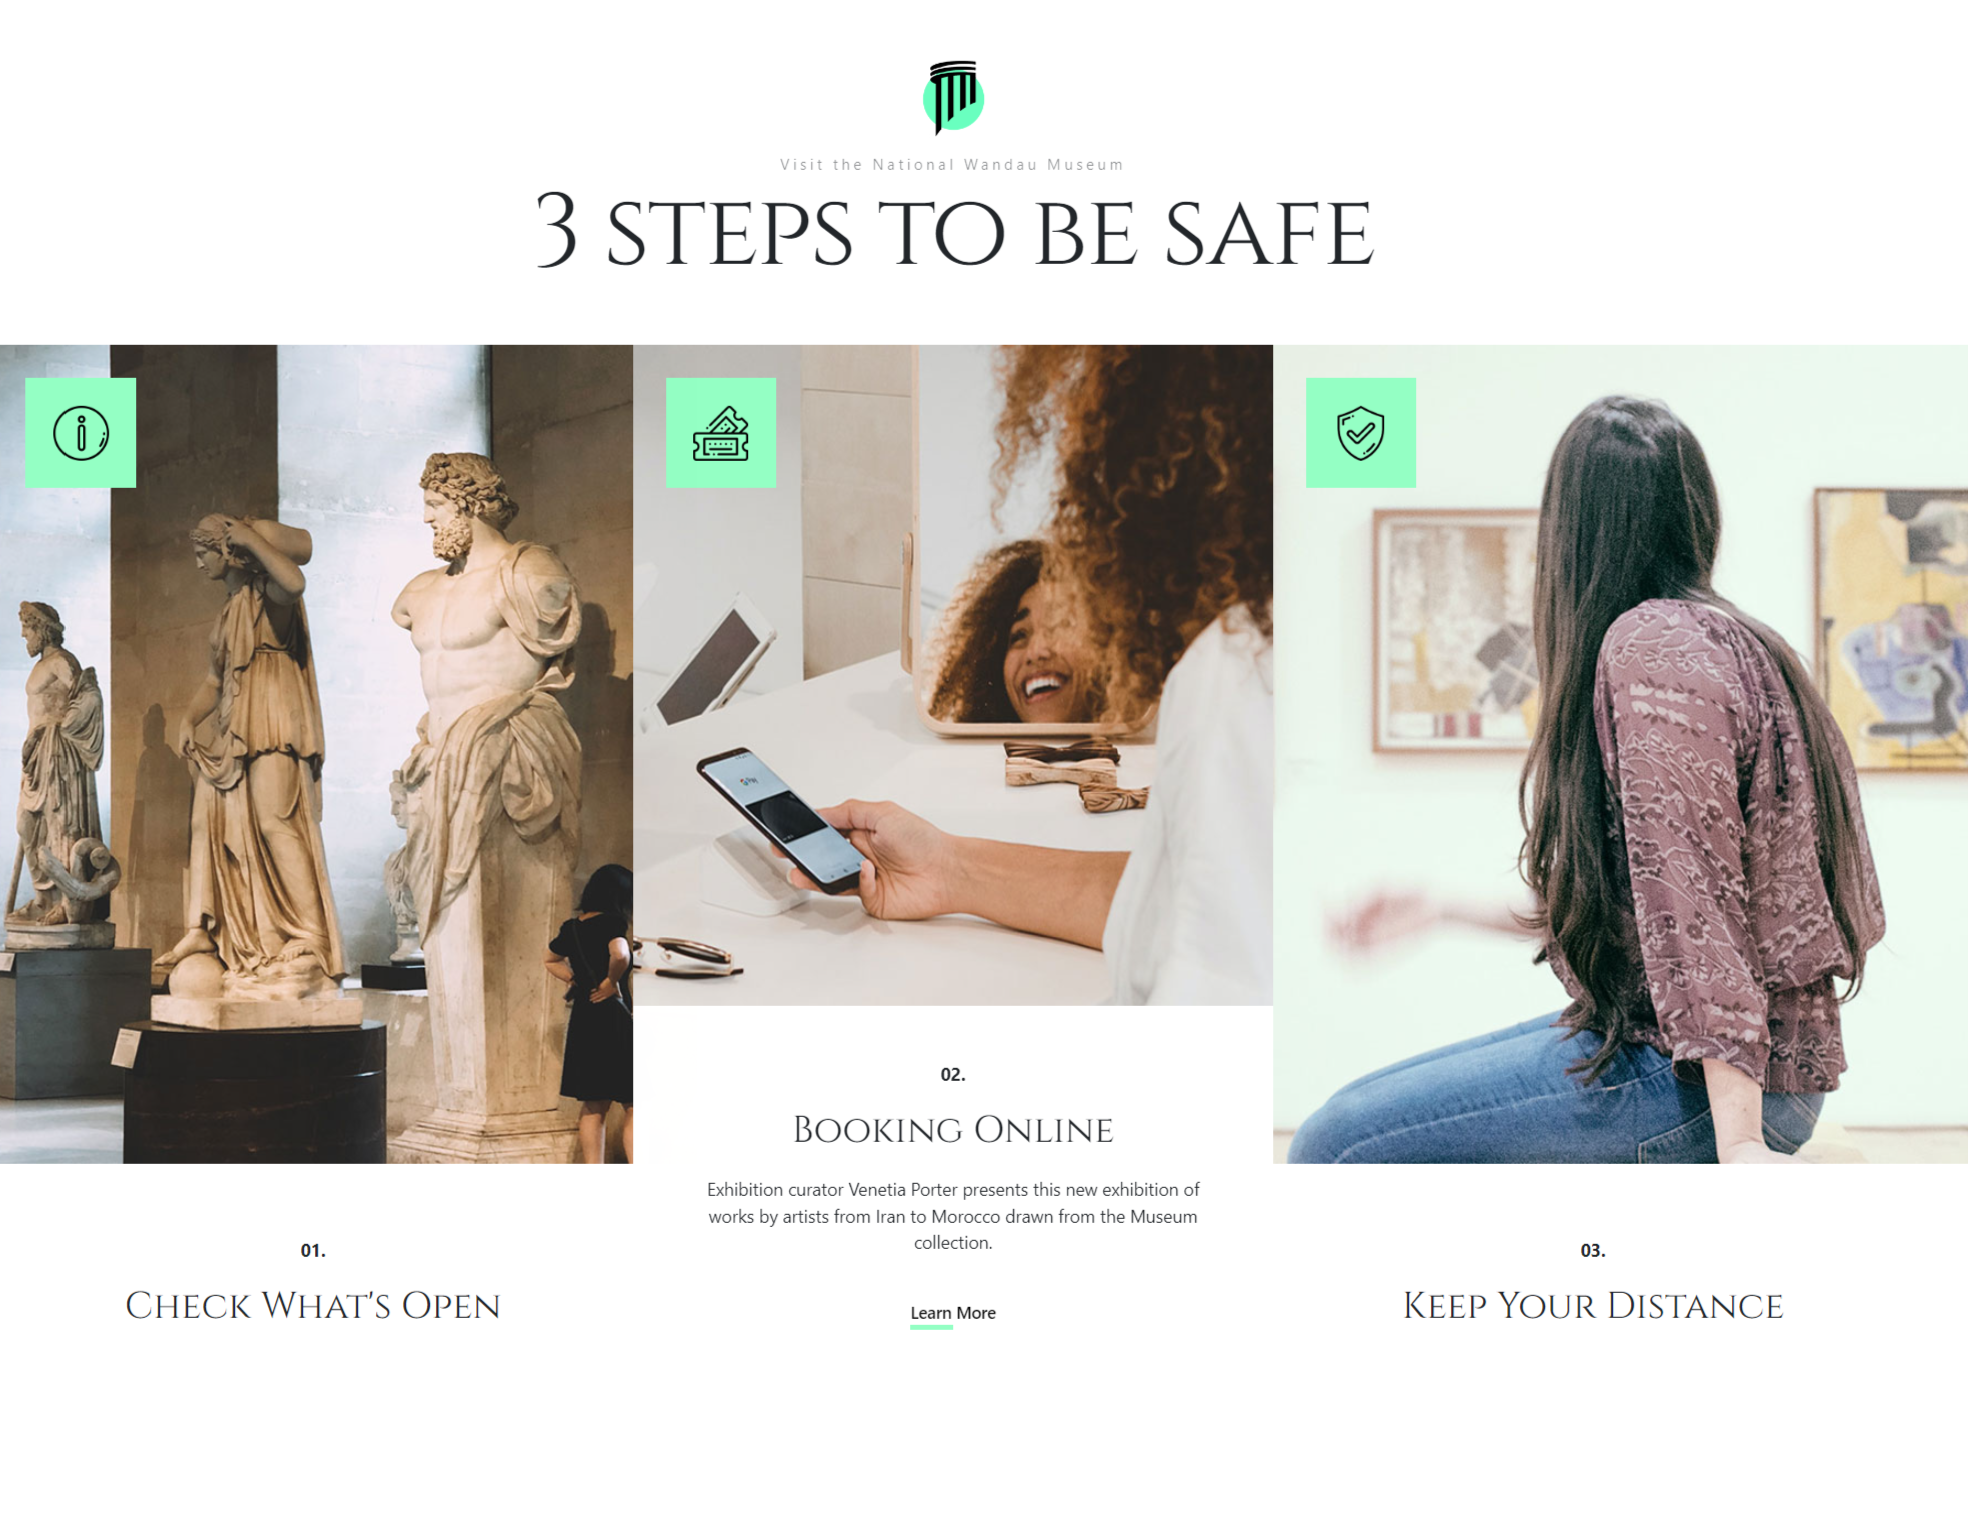
\includegraphics[width=\linewidth]{img/safety.PNG}
	\caption{Header}
	\label{fig:safety}
\end{figure} 
%%%%%%%%%%%%%%%%%%%%%%%%%%%%%%%%%%%%%%%%%%%%%%%%%%%%%%%%%%%%%%%%%%%%%%%
\section{Website Footer}
We keep our users up-to-date by sending the latest updates of our museum through emails.
Users can find us through our official links that we provided in the footer. Fig \ref{fig:footer}
\begin{figure}
	\centering
	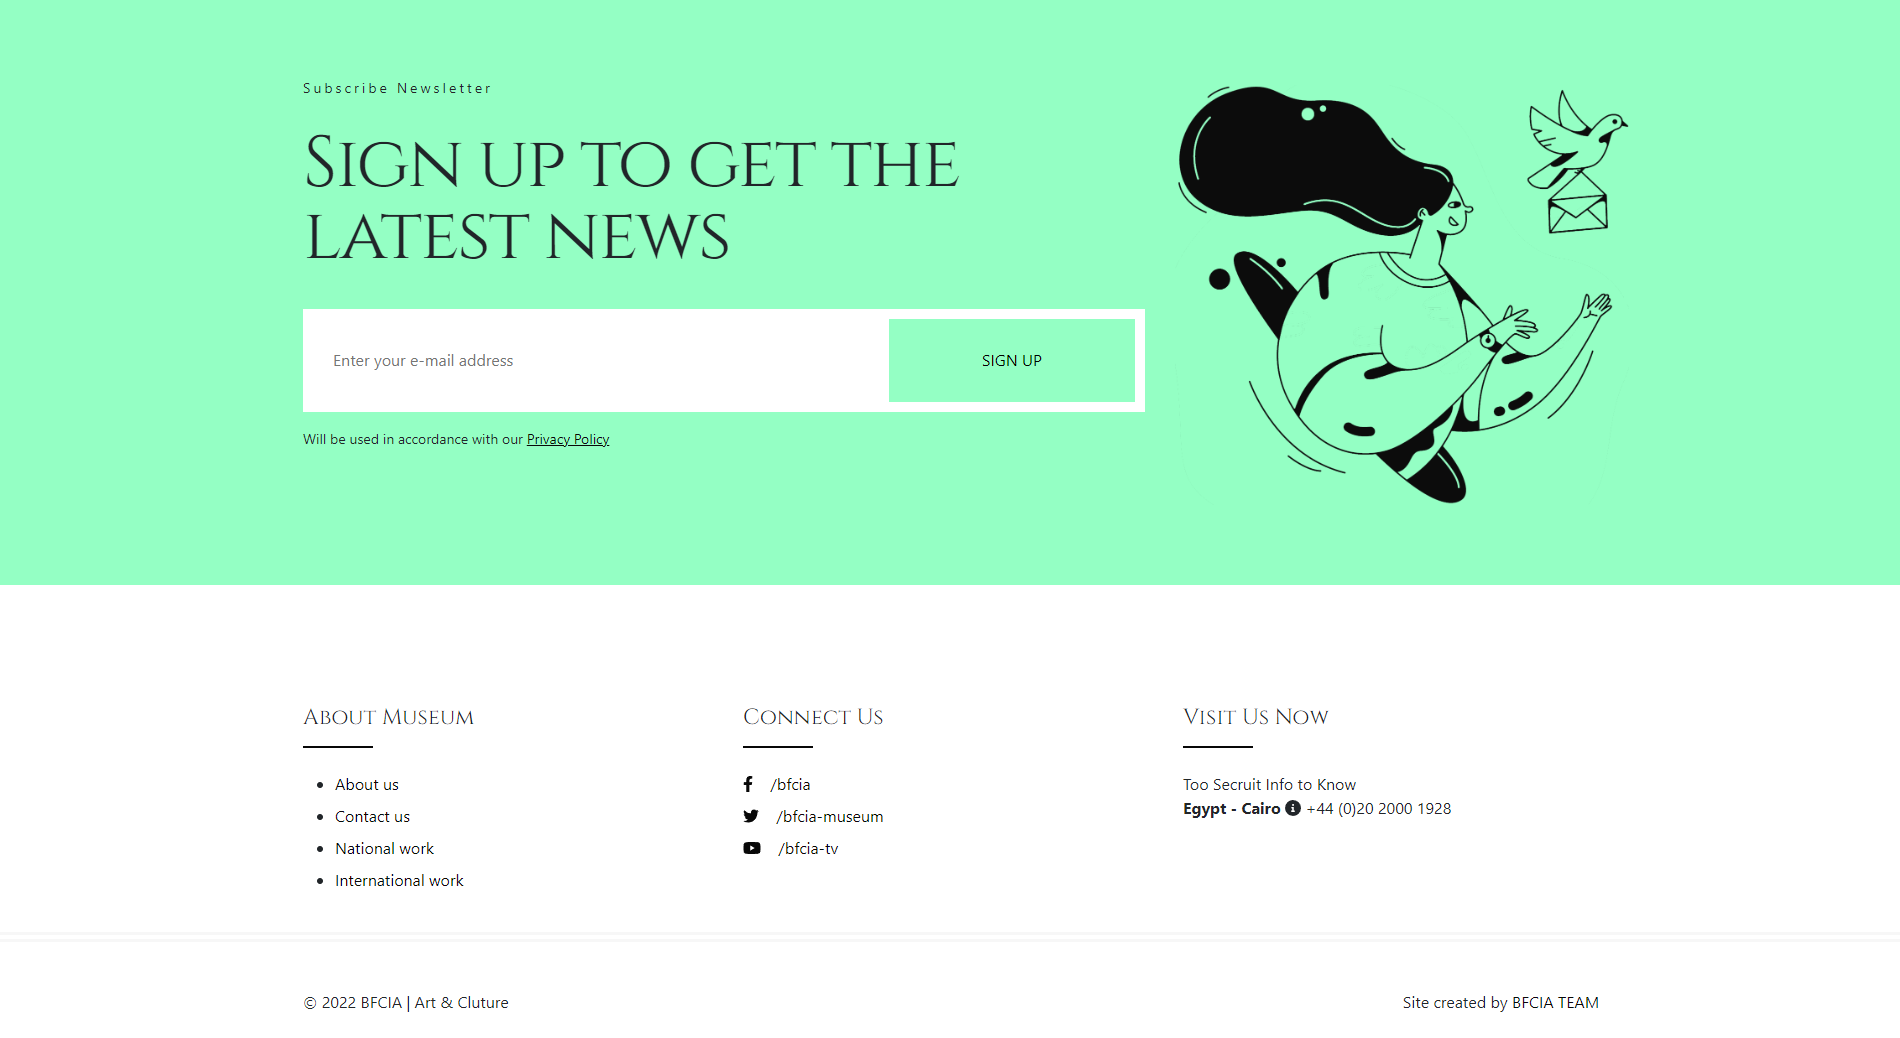
\includegraphics[width=\linewidth]{img/footer.PNG}
	\caption{Header}
	\label{fig:footer}
\end{figure} 
\end{document}


